%-------------------------------------------------------------------------
\documentclass[report,english,cleveref,autoref,a4paper]{lipics-v2021}
%-------------------------------------------------------------------------
\hideLIPIcs
\bibliographystyle{plainurl}
\usepackage{array}
\usepackage{colortbl}
\usepackage[dvipsnames]{xcolor}
\newcommand{\grayhline}{\arrayrulecolor{lightgray}\hline\arrayrulecolor{black}}
\newcommand{\graycline}[2]{\arrayrulecolor{lightgray}\cline{#1-#2}\arrayrulecolor{black}}
\nolinenumbers
%-------------------------------------------------------------------------


%-------------------------------------------------------------------------
\newcommand{\myname}{Amir Nurmukhambetov}             % your full name
\newcommand{\myshortname}{A.N.~Nurmukhambetov}             % your name with abbreviated first name(s)
\newcommand{\mystudentid}{1930907}                % put your student id here
\newcommand{\mysupervisor}{Prof.\ M.J.M.\ Roeloffzen}
\newif\ifGuidelines
\Guidelinestrue
% \textbf{}\Guidelinesfalse                                  % uncomment when submitting your portfolio
\ifGuidelines
    \newcommand{\explanation}[1]{\emph{Explanation:} #1}
\else 
    \newcommand{\explanation}[1]{}
\fi
%-------------------------------------------------------------------------


%-------------------------------------------------------------------------
\begin{document}
%-------------------------------------------------------------------------

\ifGuidelines
%-------------------------------------------------------------------------
\section*{Guidelines for Bachelor End Projects in the ALGO Cluster}
\thispagestyle{empty}
%-------------------------------------------------------------------------
This document describes the set-up of Bachelor End Projects in the ALGO cluster.
The document also provides a template for your portfolio.


%-------------------------------------------------------------------------
\subparagraph{Supervision and execution.}
%-------------------------------------------------------------------------
Bachelor End Projects (BEPs) are individual research-oriented projects.
The execution of the BEP should be done in an independent manner: the role of the
supervisor is to monitor that you do not go into the wrong direction and to give
you suggestions and feedback, not to help you solve the problem or debug your code. 

BEPs are organized in \emph{circles}: groups of up to six students with the
same supervisor and with a similar topic for their project. Each circle meets
several times with their supervisor; see below for a detailed schedule. 
During these meetings, students report on their progress and the
supervisor can give suggestions on how to proceed. Students can also learn
from other students or give them suggestions. Students may also help each other 
outside the circle meetings. However, BEPs are individual projects, so students should 
never share code or text, unless explicitly allowed by the supervisor.
When using code or other material from external sources, this should
be properly referenced in your final report.

%-------------------------------------------------------------------------
\subparagraph{Deliverables.}
%-------------------------------------------------------------------------
There are four written deliverables:
\begin{itemize}
	\item An initial \emph{project plan}, including time planning, milestones, and risk mitigation strategies. 
	\item A \emph{midterm report} on the status of the BEP after the first quartile, an updated planning, 
          and a draft version of a part of the final report. This draft version typically contains 
          most of the introduction and possibly a description of the algorithms that you have developed 
          and/or algorithms from the literature that you will use in your experiments. \emph{Discuss 
          with your supervisor what is expected from you.}
	\item The \emph{final report}, which should be at most 400 lines. See the template for
          additional guidelines.
	\item A \emph{reflection}, where you reflect on the planning, process, choices made during the project, and what you learned from it.
\end{itemize}
The fifth deliverable is the presentation, which will take place in the exam week of Q4.

The written deliverables are combined into a single \emph{portfolio} that you must submit near the end
of the course through Canvas. For archival purposes, you must also submit your initial planning, 
your midterm report, and your final report through Canvas during the course; see the schedule below for deadlines.
Note that the final portfolio must still include the initial project plan, the midterm report, and the final report.

%-------------------------------------------------------------------------
\subparagraph{Time sheets.}
%-------------------------------------------------------------------------
It is mandatory to maintain a time sheet in which you describe the activities 
you performed and how much time you spent on them during each week of 
the project. This helps you to keep track of how much time you spent on the 
project---note that you are supposed to spend about 14 hours per week on the BEP---and if the time investment 
for the various parts of the project is in line with your planning.
This is also useful at the end of the project, when you have to write a reflection.
Make your time sheets concrete. 
Here is  an example.
\\ \\
\begin{tabular}{c| m{10cm}|c}
\hline\hline
Q1: week 7  & Circle meeting & 1.5 hours \\
\cline{2-3}
     & Polished motivation and problem statement, and
     related work, in Section~1 of the final report. & 2 hours \\
\cline{2-3}
     & Finished first draft of Section 2.1 of the final report. & 6 hours \\
\cline{2-3}
     & Continued with the implementation of the greedy algorithm  & 4 hours \\
\cline{2-3}
     & \multicolumn{1}{r|}{week total} & 13.5 hours \\
\hline \hline
\end{tabular}


%-------------------------------------------------------------------------
\subparagraph{Overleaf and git.}
%-------------------------------------------------------------------------
Your portfolio must be written in \LaTeX{} using the provided template---see below---and
you must use Overleaf (\url{https://www.overleaf.com/}). You should create a new
project on Overleaf, named \texttt{ALGO-BEP-yyyy-name}, where \texttt{yyyy} is 
the current year and \texttt{name} is your last name. After creating the project
on Overleaf, you must invite your supervisor to the project. If you prefer to
edit in a different environment than in Overleaf itself, you must update
the Overleaf files every day that you have worked on the files.
There is also a separate template for the time sheets, which must be maintained in Overleaf as well
(in the same project).
\begin{quote}
\noindent \textbf{It is important that you work on your final report throughout the project:
already write the motivation and problem statement and the related-work part of
the introduction early on, write a description of your algorithms before implementing them,
and so on.}
\end{quote}
For your code you must use \url{https://gitlab.tue.nl/users/sign_in} and make sure
your supervisor has access to your repository.


%-------------------------------------------------------------------------
\subparagraph{Plagiarism and AI usage.}
%-------------------------------------------------------------------------
As already mentioned, you should not use code or text from other students
(unless explicitly allowed). The same is true for code or text from other sources:
before you use material from other sources, you must always ask permission from your supervisor.

As for AI usage: it is allowed to use AI tools to make small improvements in
the text you have written---in particular, it is allowed to use {\sc writefull} on
Overleaf---but it is not allowed to use AI tools to generate entire paragraphs.
Similarly, you can use AI tools to debug your own code or to generate small code snippets,
but not to generate long pieces of code.

%-------------------------------------------------------------------------
\subparagraph{Communication during the course.}
%-------------------------------------------------------------------------
Communication with the supervisor will mainly be done via the circle meetings.
There will also be a Slack channel for each circle. The main goal of the 
Slack channel will be to facilitate communication between students in the circle.
You may also ask questions to the supervisor in the channel, but supervisors
may not respond immediately or they may defer answering the questions to the
next circle meeting.

%-------------------------------------------------------------------------
\subparagraph{Meeting schedule.}
%-------------------------------------------------------------------------
Below is the meeting schedule for the BEPS in Q3+Q4 of the academic year 25/26.
Some remarks:
\begin{itemize}
\item Attending \emph{all} circle meetings (in person) is mandatory.
\item Deadlines for the deliverables are in \textcolor{red}{red}. These delivarables
should be submitted through the appropriate Assignment in Canvas.
\item Other ``submissions'' (draft versions, time sheets) do not have to be done through
       Canvas; just make sure that they are available through Overleaf (that is,
       make sure that your documents in Overleaf are up-to-date and contain
       the required items).
\item The weeks of the circle meetings may deviate from the general schedule below.
The exact schedule (including the day and time of the meetings) is determined by your supervisor.
\end{itemize}
%-------------------------------------------------------------------------
\begin{tabular}{c|r|l|l|l}
quartile & week & dates & meetings & deadlines for deliverables \\
\hline
Q3  & 1 & Feb 2--6 & Kickoff meeting &   \\
\graycline{2}{5}
    & 2 & Feb 9--13 & Circle meeting & \parbox[c][12mm][c]{50mm}{\textcolor{red}{Friday, Feb 13, 23:59} \\ Initial planning} \\
\graycline{2}{5}
    &  \multicolumn{4}{c}{\emph{Carnaval week}}  \\
\graycline{2}{5}
    & 3 & Feb 23--27 &  &  \\
\graycline{2}{5}
    & 4 & March 2--6 & Circle meeting & \\
\graycline{2}{5}
    & 5 &  Mar 9--13 &  & \\
\graycline{2}{5}
    & 6 & Mar 16--20 &  & \\
\graycline{2}{5}
    & 7 & Mar 23--27 & Circle meeting & \\
\graycline{2}{5}
    & 8 & Mar 30 -- Apr 3 &  &  \\
\graycline{2}{5}
    & 9 & Apr 6--10 & \emph{Exam week} & \parbox[c][17mm][c]{50mm}{\textcolor{red}{Friday, Apr 10, 23:59} \\ Midterm report \\ (including updated planning)} \\
\graycline{2}{5}
    & 10 & Apr 13--17 &  \multicolumn{2}{c}{\emph{Exam week} \hspace*{40mm}}  \\
\hline
Q4  & 1 & Apr 20--24 & Circle meeting & \\
\graycline{2}{5}
    & 2 & Apr 27 -- May 1 &  & \\
\graycline{2}{5}
    & 3 & May 4--8 &  &  \parbox[c][12mm][c]{50mm}{Friday, May 8, 23:59 \\ Draft 1.0 of final report}\\
\graycline{2}{5}
    & 4 & May 11--15 & Circle meeting & \\
\graycline{2}{5}
    & 5 & May 18--22 &  & \\
\graycline{2}{5}
    & 6 & May 25--29 &  & \\
\graycline{2}{5}
    & 7 & Jun 1--5 &  &  \parbox[c][12mm][c]{50mm}{Wednesday, June 3, 23:59 \\ Complete draft of final report} \\
\graycline{2}{5}
    & 8 & Jun 8--12  & Circle meeting & \parbox[c][12mm][c]{50mm}{\textcolor{red}{Friday, June 12, 23:59} \\ Final report}\\
\graycline{2}{5}
    & 9 & Jun 15--19  &  & \parbox[c][17mm][c]{50mm}{\textcolor{red}{Friday, June 19, 23:59} \\ Complete portfolio\\(including reflection)} \\ 
\cline{2-5}
    & 10 & Jun 22--26 &  \multicolumn{2}{c}{\emph{Exam week:} Final presentations}  \\
    & 11 & Jun 29 -- Jul 3 &  \multicolumn{2}{c}{\emph{Exam week:} Final presentations}  \\
\hline
\end{tabular}
%-------------------------------------------------------------------------


%-------------------------------------------------------------------------
\subparagraph{How to use this document as a template for your portfolio.} 
%-------------------------------------------------------------------------
To use this template, insert your full name, name with abbreviated first names,
student id, and name of your supervisor in the relevant place in the {\LaTeX} source file 
(lines 11, 12, and 13).
Before submitting, un-comment \texttt{\textbackslash{}Guidelinesfalse} on line~18.
\emph{Using the template is mandatory; do not change the document class and do not
make changes to the layout.}

\newpage
%-------------------------------------------------------------------------
\else                                           % do not show guidelines
\fi
%-------------------------------------------------------------------------

%-------------------------------------------------------------------------
\title{PORTFOLIO Bachelor Final Project (2ICS00)}
%-------------------------------------------------------------------------
\author{Student: \myname~(\mystudentid)}{Eindhoven University of Technology}{}{}{}
\author{Supervisor: \mysupervisor~(ALGO)}{$\mbox{}$}{}{}{}
\authorrunning{\myshortname}
%-------------------------------------------------------------------------

%-------------------------------------------------------------------------
\maketitle
\newpage
%-------------------------------------------------------------------------

%-------------------------------------------------------------------------
\setcounter{page}{1}
\tableofcontents
\newpage
%-------------------------------------------------------------------------

%-------------------------------------------------------------------------
\part{Process Documents}
\label{part:process}
\setcounter{page}{1}
\thispagestyle{empty}
\newpage
%-------------------------------------------------------------------------

%-------------------------------------------------------------------------
\section{Project description and initial planning (max 2 pages)}
%-------------------------------------------------------------------------

%-------------------------------------------------------------------------
\subsection{Project description}
\label{subsec:project}
%-------------------------------------------------------------------------
% \explanation{Clearly describe the problem(s) you plan to investigate, the scientific and/or
% societal or industrial relevance, and the goal(s) of the project.}

Time-constrained TSP is a variant of the Traveling Salesman Problem in which a tour must start and end at a fixed depot while staying within an upper bound~$L$ on total travel cost. Each non-depot point in the input set~$P$ is assigned a reward. The objective is to choose a subset of points and a depot-starting, depot-ending tour that maximizes collected reward while keeping the total travel cost at most~$L$.
\\ \\
In this project, I study this non-refueling TTSP variant on sparse weighted graphs. The focus is empirical: implement a fast greedy baseline, implement a genetic algorithm, use a small-instance exact solver as a reference where possible, and compare the resulting solution quality across generated instance size classes and travel budgets.

\subsubsection{Relevance}

This problem is relevant to transportation logistics. Consider a courier with a fixed travel budget, for example due to a delivery deadline, battery range, or working-hour limit. The dispatcher must choose which reward-bearing locations to visit and in what order, while ensuring that the vehicle can return to the depot within the budget. The model captures the trade-off between collecting more reward and spending more travel cost.

\subsubsection{Goal}

The goal of this project is to evaluate how much solution quality is gained by moving from a deterministic greedy baseline to a population-based genetic algorithm for the graph-based TTSP. On small instances, the heuristic rewards are compared with optimal rewards from a small-instance exact solver. On larger instances, where exact optimization is not used as the main method, results are compared against the best-known reward found among comparable result sets.

\subsubsection{Scope}

The project scope is limited to the non-refueling TTSP. It includes three computational components: a greedy insertion baseline, a genetic algorithm that searches over tour-building priorities, and a small-instance exact solver used as a reference on small datasets. Local search and refueling decisions are outside the final project scope.
\\ \\
Experiments are conducted on generated sparse graph instances and report collected reward, feasibility, travel cost, and available runtime metadata. The main comparison unit is a result set: one approach under one dataset collection, travel budget, parameter setting, and seed when applicable.

%-------------------------------------------------------------------------
\subsection{Planning}
\label{subsec:planning}
%-------------------------------------------------------------------------
% \explanation{Give a planning for the project. Make sure you include all relevant aspects (for
% experimental projects this could include: literature study, 
% design and/or theoretical analysis of algorithms, implementation of algorithms, generation of test sets,
% performing experiments, evaluation of the outcome of the experiments, writing of the final report, preparation
% of the final presentation.}

The BEP spans two quartiles (Q3 and Q4). The planning below is organized per week. I'm planning to work on report throughout the the whole process documenting steps along the way.

\subsubsection{Q3: Literature study, Greedy Heuristic, and Dataset Design}

\begin{itemize}
  \item \textbf{Week 1 -- 4: Literature Study \& Greedy Baseline}
  \begin{itemize}
    \item Study literature on the Orienteering Problem, related reward-collecting routing variants, and metaheuristics.
    \item Implement a greedy insertion heuristic based on reward gain per additional travel cost as a fast baseline.
    \item Develop core Python infrastructure: instance representation, shortest-path distance calculations, and solution I/O.
  \end{itemize}

  \item \textbf{Week 5 -- 8: Dataset Generation Design \& Midterm Report}
  \begin{itemize}
    \item Design a strategy for generating varied sparse weighted graph datasets with node rewards.
    \item Prepare the midterm report, documenting the pivot, the implemented greedy heuristic, and the updated plan for Q4.
  \end{itemize}
  
  \item \textbf{Week 9 -- 10: Buffer and Finalize Dataset Generator}
  \begin{itemize}
    \item Address any feedback from the midterm report.
    \item Finalize the Rudy-based dataset generation workflow.
  \end{itemize}
\end{itemize}

\subsubsection{Q4: Genetic Algorithm, Experiments, and Final Report}

\begin{itemize}
  \item \textbf{Week 1 -- 3: Genetic Algorithm Implementation}
  \begin{itemize}
    \item Design and implement a Genetic Algorithm (GA) that searches over candidate tour-building priorities.
    \item Test and debug GA decoding, crossover, mutation, and seeded reproducibility on small instances.
  \end{itemize}
  
  \item \textbf{Week 4 -- 6: Exact Reference and Result Infrastructure}
  \begin{itemize}
    \item Implement a small-instance exact solver to provide optimal rewards where feasible.
    \item Create reusable result-set organization, validation, and comparison scripts.
  \end{itemize}
  
  \item \textbf{Week 7 -- 8: Experimental Campaign \& Analysis}
  \begin{itemize}
    \item Run experiments comparing the greedy baseline and GA across all generated datasets.
    \item Analyze the results using exact rewards for small instances and best-known rewards for larger instances.
  \end{itemize}

  \item \textbf{Week 9 -- 10: Final Report and Presentation}
  \begin{itemize}
    \item Write the final report, detailing the algorithms, experimental setup, and results.
    \item Prepare and rehearse the final presentation.
  \end{itemize}
\end{itemize}


%-------------------------------------------------------------------------
\section{Midterm status report (max 1 page)}
%-------------------------------------------------------------------------
\textbf{Overview of Progress:}
Work so far has focused on establishing a baseline for the Time-Constrained TSP. A greedy heuristic, which iteratively inserts nodes based on the best reward gain per additional travel cost while respecting the length budget~$L$, has been implemented in Python. The necessary infrastructure for instance generation, shortest-path distance calculations on sparse graphs, and solution output is also complete.
\\ \\
\textbf{Difficulties and Pivot:}
The initial plan was to investigate a refueling variant and later to add local-search improvements. The final project scope has instead been narrowed to the standard non-refueling TTSP, with a direct comparison between a greedy baseline and a genetic algorithm. This decision was made for three main reasons:
\begin{enumerate}
    \item The refueling variant adds significant modeling complexity, while the implemented project language and experiments focus on a fixed travel budget without replenishment.
    \item Local search would introduce an additional heuristic family, but the current comparison is already meaningful with a constructive greedy baseline, a stochastic genetic algorithm, and an exact small-instance reference.
    \item A narrower scope leaves more time for careful result organization, validation, and interpretation across multiple dataset collections and travel budgets.
\end{enumerate}

\textbf{Remaining Work and Updated Planning:}
The core task for the remainder of the project is to build upon the greedy baseline. The next steps are:
\begin{enumerate}
    \item \textbf{Dataset Generation:} Generate sparse weighted graph datasets with small, medium, and large instance size classes.
    \item \textbf{Metaheuristic:} Develop a Genetic Algorithm to find high-quality feasible tours under the travel budget.
    \item \textbf{Exact Reference:} Use a small-instance exact solver to compute optimal rewards where feasible.
    \item \textbf{Experimental Evaluation:} Compare result sets from the greedy baseline and GA, using exact rewards on small instances and best-known rewards elsewhere.
\end{enumerate}

%-------------------------------------------------------------------------
\section{Reflection (max 1 page)}
%-------------------------------------------------------------------------
\explanation{Reflect on your execution of the project: What did you learn? 
Which part of the research went as you anticipated and which parts did not?
Would you do anything differently, if you had to do a similar project again?}





%-------------------------------------------------------------------------
\newpage
%-------------------------------------------------------------------------


%-------------------------------------------------------------------------
\part{Report}
\label{part:report}
%-------------------------------------------------------------------------
\newpage
%-------------------------------------------------------------------------

%-------------------------------------------------------------------------
\setcounter{section}{0}
\setcounter{page}{1}
\thispagestyle{empty}
\section*{Comparison between Heuristic Algorithms for the Time-Constrained Traveling Salesman Problem}
\textbf{\myname}

\linenumbers
%-------------------------------------------------------------------------


%-------------------------------------------------------------------------
\begin{abstract}

\explanation{Briefly describe the problem that you have studied and the main results
and conclusions of your work. Typically the abstract consists of a single
paragraph of about 5--10 lines.}

TODO

\end{abstract}
%-------------------------------------------------------------------------



%-------------------------------------------------------------------------
\section{Introduction}
\label{sec:intro}
%-------------------------------------------------------------------------
% \explanation{Typically 1.5--2 pages.}

\subparagraph{Motivation and problem statement.}

% \explanation{Give a motivation for the problem you will study. 
% Often you can do this by discussing a real-world application
% that is related to your problem.  After that, you can describe how the problem 
% can be abstracted, to arrive at your problem.
% (In some cases, it may be more appropriate to motivate the problem 
% from a purely scientific rather than an applied perspective.)
% Make sure that your problem statement is unambiguous and clear.}

Modern logistics networks increasingly demand efficient route planning
under real-world operational constraints~\cite{GRAZIASPERANZA2018830}. Consider a courier operating
a same-day delivery service: departing from a depot, the vehicle
must return before exhausting its travel budget, for example due to battery
range or working-hour regulations. Because the number of
potential delivery locations typically exceeds what can be served within
these constraints, the dispatcher must make a decision: which
subset of customers to visit, and in what order, so as to maximize the
total collected reward, whether measured in revenue, number of parcels,
or customer priority score. In this setting, the selection of delivery points
and the underlying routing problem is generally known as the
\textbf{Time-Constrained Traveling Salesman Problem} (TTSP) or the
\textbf{Orienteering Problem}. 

In the TTSP, a route must start and end at a
depot, visit only some of the available locations, and stay within a fixed travel
budget. Each non-depot location has an associated reward, and the goal is to
choose which locations to visit and in which order so that the collected reward
is as large as possible. In applications, the travel budget may represent a
maximum travel time, driving distance, battery range, or working time.

This situation is by no means unique to delivery logistics. Similar
trade-offs arise in autonomous vehicle routing~\cite{Karakostas2024}, drone-based data collection under flight-time constraints~\cite{Gaertner2022}, and mobile tourist guidance~\cite{Vansteenwegen2007},
where a tour must be planned for a visitor who can only explore a subset
of points of interest (POIs) within a limited travel budget.

In this paper, we consider a graph-based version of the TTSP. The input is an
edge-weighted graph~$G=(V,E)$, a depot~$d \in V$, a reward assigned to each
non-depot vertex, and a travel budget~$L$. A feasible tour starts and ends at
the depot, follows edges of the graph, and has total edge weight at most~$L$.
The goal is to maximize the total reward collected from visited non-depot
vertices. Unlike formulations that assume travel times are available between
every pair of locations, this graph-based formulation allows the input graph to
be incomplete; tours may only use edges present in~$E$. Rather than using exact
optimization as the main scalable method, this report studies two heuristic
approaches for this problem: a greedy insertion baseline and a genetic
algorithm. A small-instance exact solver is used as a reference on small
instances. The contribution of the work is an empirical comparison of these
approaches for graph-based TTSP instances.

\subparagraph{Related work.}
% \explanation{Discuss what is known in the literature about your problem and 
% any relevant, closely related, problems. For each paper that you discuss, 
% make it clear which problem variant they solve, 
% and try to be as explicit about the results as possible. 

% Structure the discussion in such a way that the relation between the papers is clear.
% For example, a paper may study exactly the same problem as another paper but
% obtain a better result, or they may study a more general version of the problem.}

The problem studied in this report belongs to the family of Orienteering
Problem and TTSP variants. This section introduces the different variants 
of the problem that have been defined in literature.

Several application-oriented variants extend this basic model with additional
constraints. For example, Sebastia and Marzal~\cite{MarzalSebastia2024} introduces the Team Orienteering Problem with Time Windows and Variable Profits (TOPTWVP), where each node carries a time window for service and a profit that depends on how long the vehicle spends there. Morandi et al.~\cite{MorandiLeusYaman2024} introduces the OP with multiple drones (OP-mD), where a truck and a fleet of battery-constrained drones cooperate to maximize collected prizes within a time budget. 

Feillet et al.~\cite{feillet2005traveling} survey Traveling Salesman Problems
with Profits, a closely related family of reward-collecting routing problems.
Their survey describes classical heuristic principles such as greedy insertion,
as well as metaheuristic approaches including genetic algorithms. This survey
provides the basis for the heuristic families selected in this report. This
report implements and evaluates graph-based TTSP versions of a classical
greedy-insertion principle and a genetic-algorithm-style metaheuristic on
generated sparse weighted graph instances.

\subparagraph{Contributions.}
% \explanation{Give a summary of your work, and relate it to what is known in the literature.
% This would typically be one or two paragraphs.
% \\[5mm]
% \emph{Note:} The template below is written with a project in mind that has an experimental
% component. For other types of projects, many of the guidelines given below still apply,
% but the structure would be slightly different;
% please discuss with your supervisor what is expected.}

The contribution of this thesis is an empirical study of TTSP result quality on
generated sparse weighted graph instances. The thesis implements and evaluates
two literature-grounded heuristic families: a deterministic greedy insertion
baseline and a stochastic genetic algorithm. The study focuses on how much
additional collected reward is obtained by moving from the greedy baseline to
the genetic algorithm, and where exact small-instance references or best-known
rewards can be used to interpret solution quality.

In particular, this thesis makes the following contributions:
\begin{itemize}
    \item It implements and compares a greedy insertion baseline and a genetic
    algorithm for the graph-based TTSP.
    \item It uses a small-instance exact solver as a reference for optimal
    rewards on small instances.
    \item It organizes experiments as result sets and evaluates solution
    quality across different instance size classes, travel budgets, and GA
    seeds using exact or best-known reward ratios.
\end{itemize}

%-------------------------------------------------------------------------
\section{The algorithms}
\label{sec:algorithms}
%-------------------------------------------------------------------------

%-------------------------------------------------------------------------
\subsection{Description of the algorithms}
\label{subsec:description}
%-------------------------------------------------------------------------
% \explanation{Describe the algorithms that you developed and/or relevant algorithms
% from the literature. Often this is done best using high-level (that is, not too detailed)
% pseudocode plus a textual explanation. For algorithms from the literature, discuss with 
% your supervisor in how much detail they should be presented.}

\subsubsection{Greedy Baseline}

% The implemented problem setting uses node~1 as the depot. Each node has an
% associated reward, but the depot reward is not collected. The input is an
% undirected weighted graph, and the graph is not assumed to be complete. Before
% constructing a solution, the algorithm therefore computes shortest paths between
% all pairs of nodes. When the heuristic inserts a node between two consecutive
% nodes in the current tour, that connection is interpreted as the shortest path
% between those nodes in the original graph. A tour is feasible if the total length
% of the expanded route, including the return to the depot, is at most the
% budget~$L$.

The greedy baseline follows the greedy-insertion principle described by
Feillet et al.~\cite{feillet2005traveling}: starting from the depot loop, it
repeatedly inserts the feasible node-position pair with the best reward gain per
additional travel cost. The implementation adapts this principle to sparse TTSP
instances by using shortest-path distances and by evaluating rewards on the
expanded tour. In every iteration, it considers each node that is not yet in the
selected-node tour. For each such candidate node, it tries placing the node into
each gap between two consecutive selected vertices $u$ and $v$ in the current
tour. For one candidate insertion, let $T$
denote the current shortest-path-expanded tour and let $T'$ denote the expanded
tour after inserting candidate node $x$ between $u$ and $v$. This replacement is
shown in Figure~\ref{fig:greedy-before-after-insertion}.

\begin{figure}[t]
\centering
\begin{minipage}{0.47\textwidth}
\centering
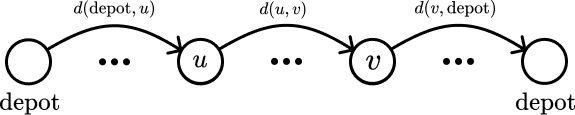
\includegraphics[width=\linewidth]{assets/before-tour.png}
\subcaption{Current tour $T$ before inserting candidate node $x$.}
\end{minipage}
\hfill
\begin{minipage}{0.47\textwidth}
\centering
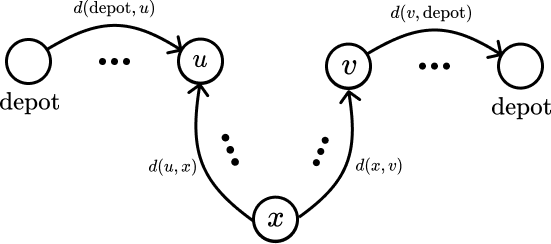
\includegraphics[width=\linewidth]{assets/after-tour.png}
\subcaption{Updated tour $T'$ after inserting $x$ between two tour vertices.}
\end{minipage}
\caption{The before and after images represent the tours $T$ and $T'$, respectively. Inserting a candidate node replaces one shortest-path segment in the selected-node tour by two shortest-path segments. The hidden intermediate vertices on these segments are part of the expanded tour.}
\label{fig:greedy-before-after-insertion}
\end{figure}

The cost effect of this insertion is the additional travel cost
\[
  \Delta C = d(u,x)+d(x,v)-d(u,v),
\]
where $d(p,q)$ is the shortest-path distance between vertices $p$ and $q$.
Insertions that would exceed the travel budget~$L$ are discarded.

The reward effect is computed after expanding the tour, not just from the reward
of node~$x$. Inserting $x$ may also add or remove intermediate nodes from the
expanded tour. The collected reward of an expanded tour is
\[
  R(T)=\sum_{\substack{u\in V(T)\\u\neq 1}} r_u,
\]
where $V(T)$ is the set of visited vertices in the expanded tour and $r_u$ is the
reward of vertex $u$. The depot is excluded, and every non-depot reward is
counted at most once. The reward gain is
\[
  \Delta R = R(T') - R(T).
\]

Using the current tour $T$ and updated tour $T'$ from
Figure~\ref{fig:greedy-before-after-insertion}, the feasible insertion is scored
as
\[
  \operatorname{score}(x,u,v) =
  \begin{cases}
    \infty, & \text{if } \Delta C = 0,\\
    \frac{\Delta R}{\Delta C}, & \text{otherwise.}
  \end{cases}
\]
The algorithm chooses the feasible insertion with the highest score. Ties are
broken deterministically by preferring the larger reward gain, then the smaller
additional travel cost, and finally the smaller node number. The selected node
is inserted into the tour, and the process repeats until no feasible insertion
with positive reward gain remains. The full construction procedure is summarized
in Appendix~\ref{app:greedy-baseline-pseudocode},
Listing~\ref{lst:greedy-baseline}.

The purpose of this heuristic is to provide a fast constructive method that
balances the benefit of visiting a node against the extra travel needed to
include it in the tour. At the same time, the method is inherently myopic,
because every decision is based only on the current tour and the locally best
insertion score. Consequently, it serves as a practical baseline, but it does
not guarantee an optimal solution.

\subsubsection{Small-Instance Exact Solver}

For small instances, I implemented an exact solver to compute an optimal reward
for the TTSP. This solver is not intended as the main scalable method. Instead,
it provides a reference point for assessing the quality of heuristic solutions
on instances where exact optimization is computationally feasible. In the
experimental evaluation, exact results are used to compute reward ratios for the
greedy baseline and the genetic algorithm on small datasets.

\subsubsection{Genetic Algorithm}

The genetic algorithm represents a candidate solution by a permutation of
non-depot nodes. This permutation is interpreted as a priority order for trying
node insertions. To evaluate one chromosome, the decoder starts from the depot
and processes nodes in chromosome order. For each node, it searches for the best
feasible insertion position in the current tour, using the same shortest-path
expanded reward accounting as the greedy baseline. If no feasible positive-gain
insertion exists for that node, the decoder skips it.
\\ \\
The initial population includes a chromosome derived from the greedy insertion
order and additional randomly shuffled chromosomes. New generations are produced
using tournament selection, order crossover, swap mutation, and elitism. The
fitness of an individual is its collected reward, with lower travel cost used as
a tie-breaker. Because the method is stochastic, experiments are run with fixed
seeds and summarized using best-of-$N$ seed summaries where multiple complete
seed result sets are available.

%-------------------------------------------------------------------------
\subsection{Analysis of the algorithms}
\label{subsec:analysis}
%-------------------------------------------------------------------------
\explanation{For each of the algorithms that you presented in Section~\ref{subsec:description}
do the following: Analyze the asymptotic running time of your algorithm(s) and, if possible,
prove their correctness. If your algorithm is a heuristic that may sometimes
fail to produce a correct solution, this should be discussed as well.
For optimization problems: discuss the quality of the solutions computed by your algorithm(s).
For algorithms from the literature: discuss with your supervisor in
how much detail you should do the analysis.}

\subsubsection{Greedy Baseline}

Let $n$ be the number of nodes and $m$ the number of edges. The preprocessing
step runs Dijkstra's algorithm from every node, which takes
$O(n(m+n)\log n)$ time when using a binary heap. The implementation also stores
the corresponding shortest paths and node-count information for reward
accounting.

During the greedy construction, at most $n-1$ nodes can be inserted into the
tour. If the current tour contains $k$ selected nodes, one iteration considers
$O(nk)$ candidate insertions. In the current implementation, evaluating a
candidate may require copying and updating node-count information and recomputing
the collected reward, which is $O(n)$ in the worst case. Summed over all
iterations, the greedy construction therefore takes $O(n^4)$ time in the worst
case after preprocessing. The heuristic always returns a feasible solution
because every accepted insertion is checked against the budget, but it is myopic:
it optimizes only the best immediate reward gain per additional travel cost and
therefore does not guarantee an optimal TTSP solution.

\subsubsection{Small-Instance Exact Solver}

The exact solver is used only as a reference method on small instances. Its role
is to compute an optimal reward for instances where doing so is practical, not to
serve as the main algorithm for all dataset sizes. This makes it useful for
quantifying heuristic quality on small instances, but unsuitable as the central
approach for medium and large generated graphs.

\subsubsection{Genetic Algorithm}

Let $P$ be the population size and $G$ the number of generations. Each
individual evaluation decodes a chromosome into a feasible tour. The decoder
uses the same insertion routine as the greedy baseline, except that it considers
nodes in chromosome order instead of always choosing the globally best immediate
insertion. In the worst case, decoding one chromosome can consider $O(n^2)$
insertions, with reward accounting costs similar to the greedy implementation.
The total running time is therefore dominated by evaluating the initial
population and all generated offspring over $G$ generations.
\\ \\
The genetic algorithm always returns a feasible tour because every decoded
insertion is checked against the travel budget. It does not guarantee an optimal
solution: crossover, mutation, and selection explore the space of priority
orders heuristically. Its advantage is that it can test many different
tour-building orders, which may overcome some of the greedy baseline's myopic
choices.

%-------------------------------------------------------------------------
\section{Experimental evaluation}
\label{sec:evaluation}
%-------------------------------------------------------------------------

%-------------------------------------------------------------------------
\subsection{Data sets}
\label{subsec:data}
%-------------------------------------------------------------------------
\explanation{Clearly describe the data sets that you use. If you use
synthetic data sets, describe how they are generated in such a way
that a reader would be able to generate the data sets themselves.
Explain the roles of the parameter(s) used to generate the data sets.
When possible and relevant, add figures of example data sets.
If you use data sets from other sources, provide a reference
to those data sets.}

Data sets are generated with Rudy, a C program for generating random graph
instances. I use its planar weighted graph generator and extend the generated
instances with node rewards. The experiments are grouped into three instance
size classes: small instances with 10 nodes, medium instances with 100 nodes,
and large instances with 1000 nodes. Each generated graph is sparse and weighted,
and each result set is evaluated under a fixed travel budget.

%-------------------------------------------------------------------------
\subsection{Experiments and discussion}
\label{subsec:experiments}
%-------------------------------------------------------------------------
The main experiment compares the greedy baseline against the genetic algorithm
on matching dataset collection and travel budget pairs. For small instances, the
small-instance exact solver provides the optimal reward, so heuristic quality is
reported as a ratio to the optimum. For medium and large instances, no exact
reference is used; instead, each solution is compared with the best-known reward
among comparable valid result sets for the same graph and travel budget.
\\ \\
Because the genetic algorithm is stochastic, multiple seeded result sets are
summarized using a best-of-$N$ seed summary when complete seeded runs are
available. This means that the GA numbers describe the strongest solution found
among those seeds for each instance, not expected single-run performance. In the
current result sets, small and medium instances use best-of-3 summaries, while
the large instance class uses best-of-1 because an additional large GA seed run
is incomplete.
\\ \\
The current aggregate results are shown in Table~\ref{tab:aggregate-results}.
The greedy baseline is already very strong on small instances. With travel
budget 30, the GA reaches the exact optimum on all 100 small instances, while
the greedy baseline reaches the optimum on 93 of them. With travel budget 100,
both methods reach the optimum on all small instances. On medium instances, the
GA provides the clearest improvement: it beats the greedy baseline in collected
reward on 81 of 100 instances and improves the mean reward ratio from 0.979 to
1.000 relative to the best-known reward. On large instances, the improvement is
much smaller: the GA beats greedy on 18 of 100 instances, ties on the remaining
82, and improves the mean reward ratio from 0.997 to 1.000.

\begin{table}[h]
\centering
\begin{tabular}{llrrrr}
\toprule
Scenario & Approach & Instances & Mean reward & Mean ratio & Wins \\
\midrule
Large, budget 100 & GA best-of-1 & 100 & 2423.8 & 1.000 & 20 \\
Large, budget 100 & Greedy & 100 & 2416.7 & 0.997 & 80 \\
Medium, budget 100 & GA best-of-3 & 100 & 1630.4 & 1.000 & 84 \\
Medium, budget 100 & Greedy & 100 & 1596.2 & 0.979 & 16 \\
Small, budget 30 & GA best-of-3 & 100 & 158.7 & 1.000 & 7 \\
Small, budget 30 & Greedy & 100 & 157.4 & 0.991 & 93 \\
Small, budget 100 & GA best-of-3 & 100 & 407.6 & 1.000 & 0 \\
Small, budget 100 & Greedy & 100 & 407.6 & 1.000 & 100 \\
\bottomrule
\end{tabular}
\caption{Aggregate comparison of the greedy baseline and genetic algorithm result sets. Ratios use exact optimum rewards for small instances and best-known rewards for medium and large instances. The wins column uses reward first, then lower travel cost and shorter route as tie-breakers.}
\label{tab:aggregate-results}
\end{table}

%-------------------------------------------------------------------------
\section{Concluding remarks}
%-------------------------------------------------------------------------
The experiments show that the greedy baseline is a strong constructive method
for the studied TTSP instances. On small instances it often reaches the exact
optimum, and with the larger travel budget it matches the exact optimum on all
tested small graphs. The genetic algorithm is most useful on medium instances,
where it improves the mean reward ratio and beats the greedy baseline on most
instances. On large instances, the current GA configuration gives only a small
average reward improvement over greedy while requiring substantially more
runtime.
\\ \\
These results support the final project scope: a direct comparison between the
greedy baseline and genetic algorithm is already informative without adding a
separate local-search component. Future work could still investigate local
search or hybrid memetic variants, but those extensions should be evaluated as a
new experiment rather than treated as part of the current thesis contribution.

%-------------------------------------------------------------------------
\bibliography{references}
%-------------------------------------------------------------------------
\explanation{Put your references in the file \texttt{references.bib}. You can cite
books~\cite{clrs-ia-2009}, journal papers~\cite{lt-stpg-79}, or
conference papers~\cite{DBLP:conf/compgeom/Chang0024}. Add a \texttt{doi} 
if possible. DBLP\footnote{\url{https://dblp.org/}} is a good source for finding reliable 
references. Note, however, that the bibtex entries in DBLP for conferences papers sometimes
contain the location and date of the conference in the title; this should be removed.}


%-------------------------------------------------------------------------
\appendix 
\newpage
%-------------------------------------------------------------------------

%-------------------------------------------------------------------------
\section{Appendix: Additional Material}             % remove if not used
%-------------------------------------------------------------------------
\explanation{In some cases it can be useful to put some material,
such as tables with additional experimental results, into an appendix.
Before adding an appendix, discuss this with your supervisor.
Note that the main text should contain all material that is important,
and that the assessment of your work will be done based on the main text.}

\subsection{Greedy Baseline Pseudocode}
\label{app:greedy-baseline-pseudocode}

\begin{lstlisting}[caption={Greedy Baseline construction procedure.},label={lst:greedy-baseline},mathescape=true]
GreedyBaseline(G, r, L, depot):
    compute shortest-path distances and paths between all node pairs
    tour <- [depot]
    expanded <- shortest-path expansion of tour

    while true:
        best <- none
        for each node x not in tour:
            for each consecutive pair (u, v) in tour:
                T_new <- expanded tour after inserting x
                DeltaC <- cost(T_new) - cost(expanded)
                if cost(expanded) + DeltaC > L:
                    continue
                DeltaR <- reward(T_new) - reward(expanded)
                if DeltaR <= 0:
                    continue
                if DeltaC = 0:
                    score <- infinity
                else:
                    score <- DeltaR / DeltaC
                key <- (score, DeltaR, -DeltaC, -x)
                best <- better of best and (key, x, pos, T_new)

        if best is none:
            break
        insert best.x into tour at best.pos
        expanded <- best.T_new

    return expanded
\end{lstlisting}

%-------------------------------------------------------------------------
\end{document}
%-------------------------------------------------------------------------
